\section{Background}\label{sec:bak}

\paragraph*{VM-based code obfuscation}
VM protection system extracts the critical code from the target program and disassembled
into native instructions, then transforms native instructions to virtual instructions.
The following, virtual instructions are encoded into bytecode program that can only be interpreted by
the special interpreter of the system itself. Virtual instructions are used to emulate native instructions,
which means that the virtual instructions set need to be able to fully implement the semantics of native instructions.
Classical VM instructions design are based on a stack machine model
where computation is performed using stack operations like push and pop.


After the code virtualized protection, a new VM section is inserted to the end of target program and the
entry point of a protected code region is redirected to a function call to the VM.
The VM section contains a bytecode program and some important VM components.
When entering the VM, component VMinit saves the native context and initializes the virtual context.
The context of the native program, which includes information such as local variables, function arguments, return address etc.,
will be stored in a VM memory space called VMContext, which consisting of a number of important virtual registers.
At the heart of the VM is an interpreter with two components: Dispatcher and handlers set.
The dispatcher fetches a bytscode from bytecode program and decodes it, then dispatches a handler to interpret it into the native code.
This process will iterate until all the bytecodes are interpreted. When exiting the VM, component VMExit restore the native context,
and the program jumps back to the native code following the critical code segment and continues to execute the rest of the program code.

The idea of VM-based code obfuscation is to use a set of bespoke bytecode instructions to
make it harder to understand how the program works by tracking the program execution.
Such protection will become invalid once the adversary figures out how bytecodes are mapped into native code.

\begin{figure}[t]%
    \centering
    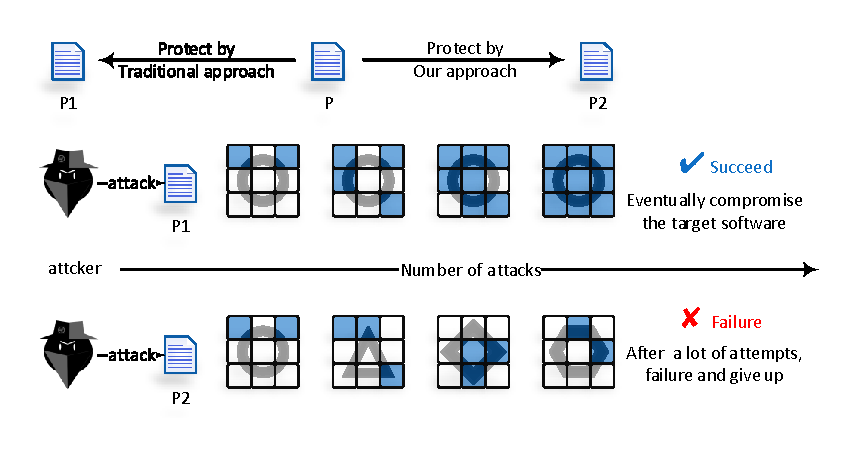
\includegraphics[width=0.7\columnwidth]{figure/figone.pdf}
    \caption{Diversity affects effectiveness of the attack. In this example, a dark small square represents reusable attacking knowledge. Diverse program execution increases the difficulty of attacks.}\label{fig:Fig.1}
    %\vspace{-5mm}
\end{figure}

\paragraph*{Cumulative attacks}
Figure~\ref{fig:Fig.1} illustrates how an attacker
can reuse knowledge extracted from the previous runs of the same application or
other applications (that are protected using the same VM scheme) to perform attack.
This is referred as \emph{cumulative attacks} in this paper.
In the first scenario, the software always follows the same execution path
across multiple runs, and a few runs will allow an attacker to
obtain sufficient knowledge about the program behavior.
In the second scenario, the program execution path changes across different runs.
As such, it will take longer and many more runs to gather enough information to perform the attack.
As can be seen from this simple illustration, diversity keys to protect against dynamic cumulative attacks.
This work aims to achieve this purpose.
